

\newcommand{\graphscale}{0.7}

\begin{figure}
  \centering
  \begin{subfigure}[c]{0.22\textwidth}
    \centering
    \scalebox{\graphscale}{
    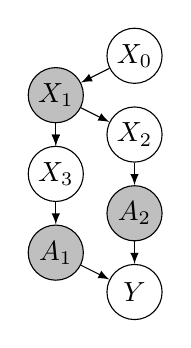
\begin{tikzpicture}[mynode/.style={circle,draw=black,fill=white,inner sep=0pt,minimum size=0.7cm},>=latex]
      \node[mynode] (x0) at (1,0.5) {$X_{0}$};
      \node[mynode][fill=lightgray] (x1) at (0,0) {$X_{1}$};
      \node[mynode] (x2) at (1,-0.5) {$X_{2}$};
      \node[mynode] (x3) at (0,-1) {$X_{3}$};
      \node[mynode][fill=lightgray] (a1) at (0,-2) {$A_{1}$};
      \node[mynode][fill=lightgray] (a2) at (1,-1.5) {$A_{2}$};
      \node[mynode] (y) at (1,-2.5) {$Y$};

      \draw[->] (x0) -- (x1);
      \draw[->] (x1) -- (x2);
      \draw[->] (x1) -- (x3);
      \draw[->] (x1) -- (x3);
      \draw[->] (x3) -- (a1);
      \draw[->] (x2) -- (a2);
      \draw[->] (a1) -- (y);
      \draw[->] (a2) -- (y);
    \end{tikzpicture}
  } %
    \caption{Two parents with a lowest common ancestor. It may happen that setting $X_{1}$ a certain value will set $(A_{1}, A_{2})$ to $(a_{1}^{*},a_{2}^{*})$, while intervening on one of the $A_{i}$ would not.}
    \label{subfig:twopar_heur}
  \end{subfigure}
  \hfill
  \begin{subfigure}[c]{0.22\textwidth}
    \centering
    \scalebox{\graphscale}{
      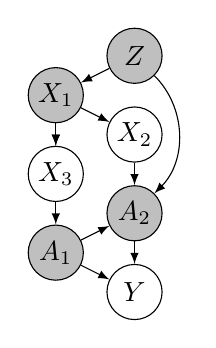
\begin{tikzpicture}[mynode/.style={circle,draw=black,fill=white,inner sep=0pt,minimum size=0.7cm},>=latex]
      \node[mynode][fill=lightgray] (z) at (1,0.5) {$Z$};
      \node[mynode][fill=lightgray] (x1) at (0,0) {$X_{1}$};
      \node[mynode] (x2) at (1,-0.5) {$X_{2}$};
      \node[mynode][fill=white] (x3) at (0,-1) {$X_{3}$};
      \node[mynode][fill=lightgray] (a1) at (0,-2) {$A_{1}$};
      \node[mynode][fill=lightgray] (a2) at (1,-1.5) {$A_{2}$};
      \node[mynode] (y) at (1,-2.5) {$Y$};

      \draw[->] (z) -- (x1);
      \draw[->] (z.south east) to [out=315,in=45,looseness=1.0] (a2.north east);
      \draw[->] (x1) -- (x2);
      \draw[->] (x1) -- (x3);
      \draw[->] (x1) -- (x3);
      \draw[->] (x3) -- (a1);
      \draw[->] (x2) -- (a2);
      \draw[->] (a1) -- (y);
      \draw[->] (a1) -- (a2);
      \draw[->] (a2) -- (y);
    \end{tikzpicture}
  }
    \caption{The heuristics justifying the need to test the LSCA $X_{1}$ of the parents $A_{1}, A_{2}$ of $Y$ can be repeated for $X_{1}$ and $A_{2}$. Thus, $Z$ should be tested as well.}
    \label{subfig:not_lca_heur}
  \end{subfigure}
  \begin{subfigure}[c]{0.22\textwidth}
    \centering
    \scalebox{\graphscale}{
    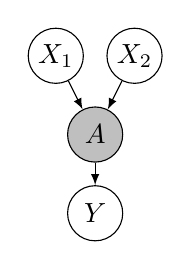
\begin{tikzpicture}[mynode/.style={circle,draw=black,fill=white,inner sep=0pt,minimum size=0.7cm},>=latex]
      \node[mynode] (x1) at (-0.5,-0.5) {$X_{1}$};
      \node[mynode] (x2) at (0.5,-0.5) {$X_{2}$};
      \node[mynode][fill=lightgray] (a) at (0,-1.5) {$A$};
      \node[mynode] (y) at (0,-2.5) {$Y$};

      \draw[->] (x1) -- (a);
      \draw[->] (x2) -- (a);
      \draw[->] (a) -- (y);
    \end{tikzpicture}
    } %
    \caption{Single parent. Setting $A$ to $a^{*}$ is the best option.}
    \label{subfig:one-parent-heur}
  \end{subfigure}
  \hfill
  \begin{subfigure}[c]{0.22\textwidth}
    \centering
    \scalebox{\graphscale}{
    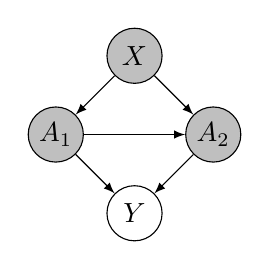
\begin{tikzpicture}[mynode/.style={circle,draw=black,fill=white,inner sep=0pt,minimum size=0.7cm},>=latex]
      \node[mynode][fill=lightgray] (x) at (0,-0.5) {$X$};
      \node[mynode][fill=lightgray] (a1) at (-1.0,-1.5) {$A_{1}$};
      \node[mynode][fill=lightgray] (a2) at (1.0,-1.5) {$A_{2}$};
      \node[mynode] (y) at (0,-2.5) {$Y$};

      \draw[->] (x) -- (a1);
      \draw[->] (x) -- (a2);
      \draw[->] (a1) -- (a2);
      \draw[->] (a1) -- (y);
      \draw[->] (a2) -- (y);
    \end{tikzpicture}
    } %
    \caption{Just as in \Cref{subfig:twopar_heur}, $X$ may need to be intervened upon. However, $\LCA(A_{1}, A_{2})=\{A_{1}\} \not\ni X$.}
    \label{subfig:vanilla-lca-issue}
  \end{subfigure}

  \caption{Examples illustrating heuristics behind the graphical characterization of the minimal interventionally superior set. The gray nodes are those that should be tested by conditional causal bandit algorithms.}
\end{figure}
